\documentclass[aspectratio=169]{beamer}

% University of Basel Beamer Style
\usepackage{unibas-beamer}

% Presentation metadata
\title{TraceGuard: Taint-Guided Symbolic Execution}
\subtitle{Bachelor Thesis Presentation}
\author{Ruben Hutter}
\date{\today}
\institute[CS]{University of Basel, Faculty of Science \\ Department of Mathematics and Computer Science}

% University logo (adjust path as needed)
\titlegraphic{%
    \vspace*{4.2cm}\hspace*{0.70\linewidth}%
    
\includegraphics[width=4cm]{./thm/picLogo}
}

\begin{document}

\maketitle

\begin{frame}
    \frametitle{Today's Journey}
    \begin{enumerate}
        \item \textbf{The Challenge:} Software vulnerabilities and current detection limits
        \item \textbf{The Problem:} Why symbolic execution struggles
        \item \textbf{The Insight:} Taint-guided exploration concept
        \item \textbf{The Solution:} TraceGuard's approach and implementation
        \item \textbf{The Evidence:} Evaluation results and performance gains
        \item \textbf{Seeing It Work:} Live demonstration
        \item \textbf{Looking Forward:} Future directions and broader impact
    \end{enumerate}
\end{frame}

\section{The Problem}

\begin{frame}
    \frametitle{Where Do Software Vulnerabilities Actually Hide?}
    \vspace{1em}
    \begin{columns}
        \begin{column}{0.5\textwidth}
            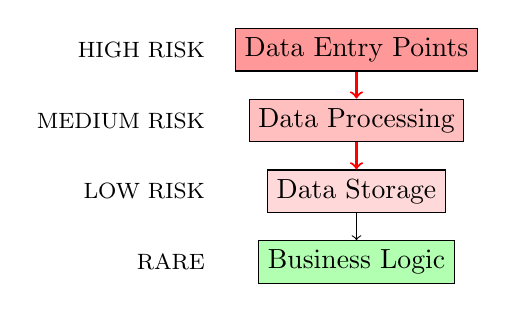
\begin{tikzpicture}[scale=0.9]
                \node[draw, rectangle, fill=red!40] (entry) at (0,3.5) {Data Entry Points};
                \node[draw, rectangle, fill=red!25] (processing) at (0,2.5) {Data Processing};
                \node[draw, rectangle, fill=red!15] (storage) at (0,1.5) {Data Storage};
                \node[draw, rectangle, fill=green!30] (logic) at (0,0.5) {Business Logic};
                
                \draw[->, thick, red] (entry) -- (processing);
                \draw[->, thick, red] (processing) -- (storage);
                \draw[->] (storage) -- (logic);
                
                \node[left] at (-2,3.5) {\footnotesize HIGH RISK};
                \node[left] at (-2,2.5) {\footnotesize MEDIUM RISK};
                \node[left] at (-2,1.5) {\footnotesize LOW RISK};
                \node[left] at (-2,0.5) {\footnotesize RARE};
            \end{tikzpicture}
        \end{column}
        \begin{column}{0.5\textwidth}
            \textbf{Vulnerability Hotspots:}
            \begin{itemize}
                \item \textbf{Data Entry:} Network I/O, file parsing, user input
                \item \textbf{Data Processing:} String operations, format parsing, validation
                \item \textbf{Data Storage:} Memory allocation, buffer operations
                \item \textbf{Business Logic:} Complex algorithms, decision trees
            \end{itemize}
        \end{column}
    \end{columns}
    
    \vspace{1em}
    \begin{center}
        \large\alert{Risk decreases as data moves away from external sources}
    \end{center}
\end{frame}

\begin{frame}
    \frametitle{Common Vulnerability Patterns}
    \vspace{1em}
    \begin{columns}
        \begin{column}{0.5\textwidth}
            \textbf{Input-Related Vulnerabilities:}
            \begin{itemize}
                \item \textbf{Buffer overflows:} \texttt{strcpy(small\_buf, user\_input)}
                \item \textbf{Format string bugs:} \texttt{printf(user\_string)}
                \item \textbf{Injection attacks:} SQL, command injection
                \item \textbf{Integer overflows:} Size calculations from input
            \end{itemize}
        \end{column}
        \begin{column}{0.5\textwidth}
            \textbf{Example Attack Flow:}
            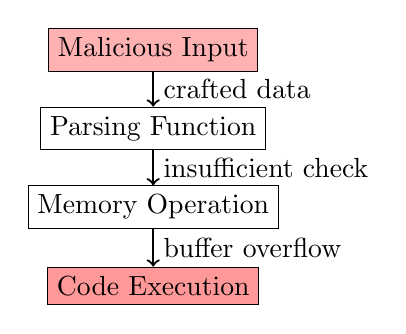
\begin{tikzpicture}[scale=1]
                \node[draw, rectangle, fill=red!30] (input) at (0,3) {Malicious Input};
                \node[draw, rectangle] (parse) at (0,2) {Parsing Function};
                \node[draw, rectangle] (memory) at (0,1) {Memory Operation};
                \node[draw, rectangle, fill=red!40] (exploit) at (0,0) {Code Execution};
                
                \draw[->, thick] (input) -- node[right] {crafted data} (parse);
                \draw[->, thick] (parse) -- node[right] {insufficient check} (memory);
                \draw[->, thick] (memory) -- node[right] {buffer overflow} (exploit);
            \end{tikzpicture}
        \end{column}
    \end{columns}
    
    \vspace{1em}
    \begin{center}
        \textbf{Key Insight:} Following the data flow from input to vulnerability
    \end{center}
\end{frame}

\begin{frame}
    \frametitle{The Challenge: Finding These Vulnerabilities}
    \vspace{1em}
    \begin{columns}
        \begin{column}{0.5\textwidth}
            \textbf{Traditional Testing Approaches:}
            \begin{itemize}
                \item \textbf{Manual code review:} Time-intensive, incomplete coverage
                \item \textbf{Unit testing:} Limited to expected inputs
                \item \textbf{Integration testing:} Misses edge cases
                \item \textbf{Static analysis:} High false positive rates
            \end{itemize}
        \end{column}
        \begin{column}{0.5\textwidth}
            \begin{tikzpicture}[scale=1]
                \node[draw, ellipse, fill=red!30] (malicious) at (0,3) {Malicious Inputs};
                \node[draw, ellipse, fill=yellow!30] (edge) at (0,2) {Edge Cases};
                \node[draw, ellipse, fill=blue!30] (normal) at (0,1) {Normal Inputs};
                \node[draw, rectangle] (testing) at (0,-0.2) {Traditional Testing};
                
                \draw[->] (testing.west) to[out=120,in=240] (normal.west);
                \draw[->, dashed] (testing.west) to[out=150,in=210] (edge.west);
                \draw[->, red, very thick, dashed] (testing.east) to[out=0,in=0] node[right] {\footnotesize missed} (malicious.east);
            \end{tikzpicture}
        \end{column}
    \end{columns}
    \vspace{1em}
    \textbf{The Gap:} Security vulnerabilities often trigger under specific, unexpected input conditions
\end{frame}

\begin{frame}
    \frametitle{Symbolic Execution - The Promise}
    \begin{columns}
        \begin{column}{0.6\textwidth}
            \textbf{Goal:} Find all possible bugs automatically
            
            \vspace{0.5em}
            \textbf{Method:} Treat inputs as mathematical symbols
            
            \vspace{0.5em}
            \textbf{Power:} Can generate test cases for any reachable code
            
            \vspace{0.5em}
            \textbf{Advantage:} Handles complex conditions that random testing cannot reach
        \end{column}
        \begin{column}{0.4\textwidth}
            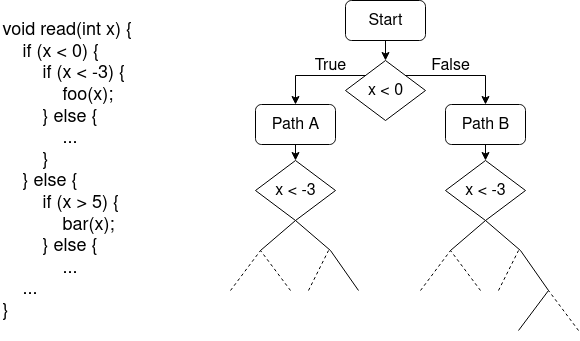
\includegraphics[width=\textwidth]{./pic/symbolic_execution_promise.png}
        \end{column}
    \end{columns}
    
    \vspace{1em}
    \begin{center}
        \large\textbf{Instead of testing with specific values, explore ALL possible values}
    \end{center}
\end{frame}

\begin{frame}
    \frametitle{The Reality - Path Explosion Problem}
    \begin{columns}
        \begin{column}{0.6\textwidth}
            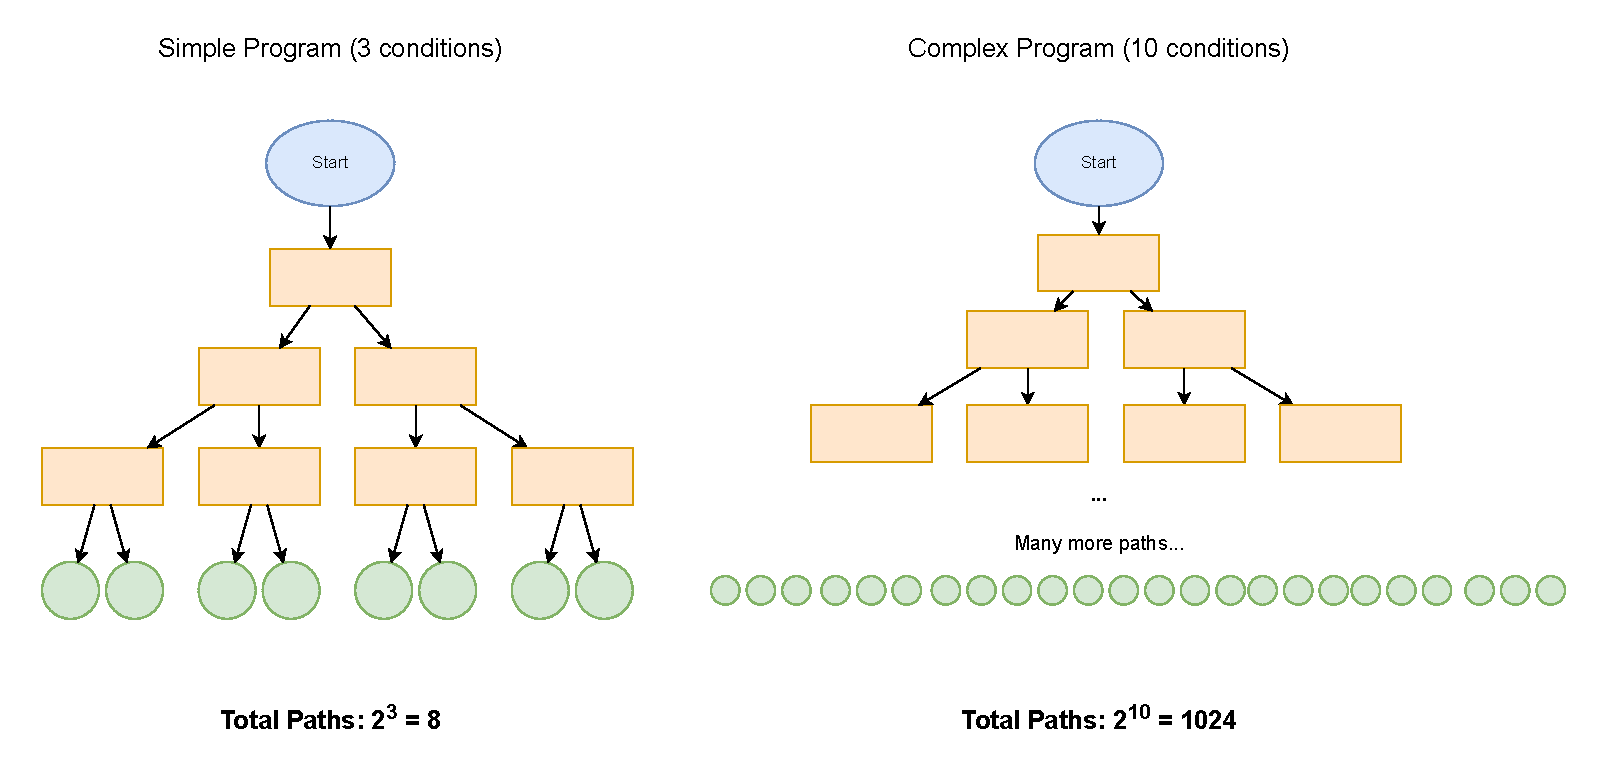
\includegraphics[width=\textwidth]{./pic/path_explosion_problem.pdf}
        \end{column}
        \begin{column}{0.4\textwidth}
            \begin{itemize}
                \item 3 conditions $\to$ 8 possible paths
                \item 10 conditions $\to$ 1,024 possible paths  
                \item 20 conditions $\to$ 1,048,576 possible paths
                \item \alert{Real programs:} Millions of conditions = computational infeasibility
            \end{itemize}
        \end{column}
    \end{columns}
    
    \vspace{1em}
    \begin{center}
        \large\alert{Exponential growth kills practical application}
    \end{center}
\end{frame}

\begin{frame}
    \frametitle{Comparing Approaches - Fuzzing vs. Symbolic Execution}
    \begin{table}[]
        \centering
        \begin{tabular}{@{}ll@{}}
        \toprule
        \textbf{Fuzzing} & \textbf{Symbolic Execution} \\
        \midrule
        Fast, lightweight & Slow, resource-intensive \\
        Shallow bug discovery & Deep path exploration \\
        Random/guided input generation & Systematic path coverage \\
        Struggles with complex conditions & Handles complex logic well \\
        \bottomrule
        \end{tabular}
    \end{table}
    
    \begin{research}{Challenge}
        Both struggle with scale, but in different ways:
        \begin{itemize}
            \item \textbf{Fuzzing:} Hard to reach deep code paths
            \item \textbf{Symbolic Execution:} Exponential path explosion
        \end{itemize}
    \end{research}
    
    \begin{center}
        \textbf{We need the systematic power of symbolic execution with better efficiency}
    \end{center}
\end{frame}

\section{The Insight}

\begin{frame}
    \frametitle{The Core Insight - Taint as a Guide}
    \vspace{1em}
    \begin{columns}
        \begin{column}{0.5\textwidth}
            \textbf{Classical Exploration:}
            \begin{center}
            \begin{tikzpicture}[scale=1]
                \node[draw, ellipse] (start) at (0,3) {Start};
                \node[draw, rectangle] (all1) at (-2,2) {Path 1};
                \node[draw, rectangle] (all2) at (0,2) {Path 2};
                \node[draw, rectangle] (all3) at (2,2) {Path 3};
                \node[draw, ellipse] (end1) at (-2,1) {End};
                \node[draw, ellipse] (end2) at (0,1) {End};
                \node[draw, ellipse] (end3) at (2,1) {End};
                
                \draw[->] (start) -- (all1);
                \draw[->] (start) -- (all2);
                \draw[->] (start) -- (all3);
                \draw[->] (all1) -- (end1);
                \draw[->] (all2) -- (end2);
                \draw[->] (all3) -- (end3);
                
                \node at (0,0) {\footnotesize Explores everything};
            \end{tikzpicture}
            \end{center}
        \end{column}
        \begin{column}{0.5\textwidth}
            \textbf{Taint-Guided Exploration:}
            \begin{center}
            \begin{tikzpicture}[scale=1]
                \node[draw, ellipse] (start) at (0,3) {Start};
                \node[draw, rectangle, fill=red!30] (taint1) at (-2,2) {Tainted};
                \node[draw, rectangle] (safe2) at (0,2) {Safe};
                \node[draw, rectangle, fill=red!30] (taint3) at (2,2) {Tainted};
                \node[draw, ellipse, fill=red!30] (vuln1) at (-2,0.9) {Vuln!};
                \node[draw, ellipse] (end2) at (0,1) {End};
                \node[draw, ellipse, fill=red!30] (vuln3) at (2,0.9) {Vuln!};
                
                \draw[->, thick, red] (start) -- (taint1);
                \draw[->] (start) -- (safe2);
                \draw[->, thick, red] (start) -- (taint3);
                \draw[->, thick, red] (taint1) -- (vuln1);
                \draw[->] (safe2) -- (end2);
                \draw[->, thick, red] (taint3) -- (vuln3);
                
                \node at (0,0) {\footnotesize Follows the data};
            \end{tikzpicture}
            \end{center}
        \end{column}
    \end{columns}
    
    \begin{implementation}{Key Realization}
        \begin{itemize}
            \item Not all execution paths are equally likely to contain vulnerabilities
            \item Paths processing user-controlled data deserve priority
        \end{itemize}
    \end{implementation}
\end{frame}

\begin{frame}[fragile]
    \frametitle{What is Taint Analysis?}
    \vspace{1em}
    \begin{columns}
        \begin{column}{0.5\textwidth}
            \textbf{Definition:} Track data derived from untrusted sources
            
            \begin{itemize}
                \item \textbf{Sources:} User input functions (fgets, scanf, network recv)
                \item \textbf{Propagation:} Through assignments, function calls, memory operations
                \item \textbf{Sinks:} Security-sensitive operations (strcpy, system calls)
            \end{itemize}
        \end{column}
        \begin{column}{0.5\textwidth}
            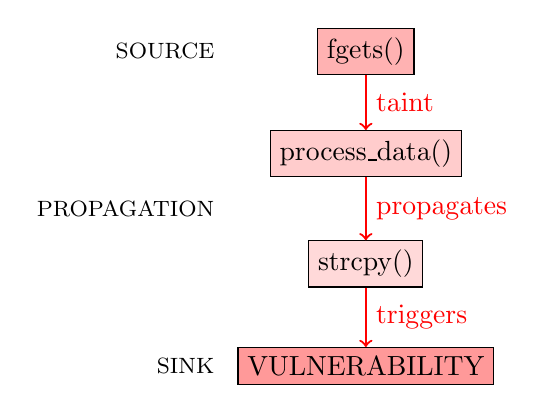
\begin{tikzpicture}[scale=1]
                \node[draw, rectangle, fill=red!30] (source) at (0,4) {fgets()};
                \node[draw, rectangle, fill=red!20] (prop1) at (0,2.7) {process\_data()};
                \node[draw, rectangle, fill=red!15] (prop2) at (0,1.3) {strcpy()};
                \node[draw, rectangle, fill=red!40] (sink) at (0,0) {VULNERABILITY};
                
                \draw[->, thick, red] (source) -- node[right] {taint} (prop1);
                \draw[->, thick, red] (prop1) -- node[right] {propagates} (prop2);
                \draw[->, thick, red] (prop2) -- node[right] {triggers} (sink);
                
                \node[left] at (-1.8,4) {\footnotesize SOURCE};
                \node[left] at (-1.8,2) {\footnotesize PROPAGATION};
                \node[left] at (-1.8,0) {\footnotesize SINK};
            \end{tikzpicture}
        \end{column}
    \end{columns}
    
    \vspace{1em}
    \begin{lstlisting}[language=C]
char buffer[100];
fgets(buffer, 100, stdin);  // TAINT SOURCE
process_data(buffer);       // TAINT PROPAGATES  
strcpy(dest, buffer);       // POTENTIAL VULNERABILITY
    \end{lstlisting}
\end{frame}

\begin{frame}
    \frametitle{Traditional Approach vs. TraceGuard}
    \vspace{1em}
    \begin{columns}
        \begin{column}{0.5\textwidth}
            \textbf{Traditional Symbolic Execution:}
            \begin{itemize}
                \item Explore all paths uniformly
                \item Hope to eventually reach vulnerable code
                \item Often times out before finding bugs
                \item Wastes resources on irrelevant paths
            \end{itemize}
        \end{column}
        \begin{column}{0.5\textwidth}
            \textbf{TraceGuard's Taint-Guided Approach:}
            \begin{itemize}
                \item Real-time taint tracking during symbolic execution
                \item Dynamic prioritization based on taint interaction
                \item Focus computational resources on security-relevant paths
                \item Find more vulnerabilities with focused exploration
            \end{itemize}
        \end{column}
    \end{columns}
    
    \vspace{1em}
    \begin{center}
        \large\textbf{Key Innovation: Integration, not post-processing}
    \end{center}
\end{frame}

\section{The Solution}

\begin{frame}
    \frametitle{TraceGuard Architecture - Overview}
    \vspace{1em}
    \begin{tikzpicture}[node distance=1.5cm]
        \node[draw, rectangle, fill=UnibasMint!30] (binary) at (0,4) {Binary Program (C/C++, AMD64)};
        \node[draw, rectangle, fill=UnibasBlue!30] (phase1) at (0,3) {Phase 1: Static Analysis \& Function ID};
        \node[draw, rectangle, fill=UnibasPurple!30] (phase2) at (0,2) {Phase 2: Dynamic Taint Tracking};
        \node[draw, rectangle, fill=UnibasMintDark!30] (phase3) at (0,1) {Phase 3: Guided Symbolic Execution};
        \node[draw, rectangle, fill=green!30] (output) at (0,0) {Vulnerabilities \& Visualization};
        
        \draw[->] (binary) -- (phase1);
        \draw[->] (phase1) -- (phase2);
        \draw[->] (phase2) -- (phase3);
        \draw[->] (phase3) -- (output);
        
        \node[right] at (4,3) {CFG construction, function hooks};
        \node[right] at (4,2) {Real-time taint propagation};
        \node[right] at (4,1) {Priority-based state exploration};
    \end{tikzpicture}
    
    \vspace{1em}
    \begin{implementation}{Integration Point}
        \begin{itemize}
            \item Built on Angr symbolic execution framework
        \end{itemize}
    \end{implementation}
\end{frame}

\begin{frame}
    \frametitle{How TraceGuard Works - Function Hooking}
    \vspace{1em}
    \begin{columns}
        \begin{column}{0.5\textwidth}
            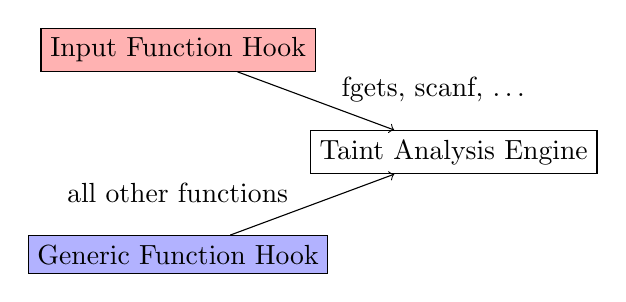
\begin{tikzpicture}[scale=1]
                \node[draw, rectangle, fill=red!30] (input) at (0,3.8) {Input Function Hook};
                \node[draw, rectangle] (analysis) at (3.5,2.5) {Taint Analysis Engine};
                \node[draw, rectangle, fill=blue!30] (generic) at (0,1.2) {Generic Function Hook};
                
                \draw[->] (input) -- node[above, right, pos=0.3, xshift=6mm] {fgets, scanf, \dots} (analysis);
                \draw[->] (generic) -- node[above, left, pos=0.7, xshift=-6mm] {all other functions} (analysis);
            \end{tikzpicture}
        \end{column}
        \begin{column}{0.5\textwidth}
            \textbf{Function Hooking Strategy:}
            \begin{itemize}
                \item \textbf{Input Function Hooks:} Detect taint introduction
                \item \textbf{Generic Function Hooks:} Monitor taint propagation
                \item \textbf{Real-time Detection:} Analyze register/memory contents
                \item \textbf{Taint Marking:} Create symbolic variables with taint IDs
            \end{itemize}
        \end{column}
    \end{columns}
    
    \vspace{1em}
    \textbf{Example:} When \texttt{fgets()} is called → Create \texttt{"taint\_source\_fgets\_001"} symbolic variable
\end{frame}

\begin{frame}
    \frametitle{Dynamic State Scoring Algorithm}
    \vspace{1em}
    \begin{columns}
        \begin{column}{0.5\textwidth}
            \begin{tikzpicture}[scale=1]
                \node[draw, rectangle] (state) at (0,4.5) {Execution State};
                \node[draw, diamond, aspect=3] (taint) at (0,3) {Taint Interaction?};
                \node[draw, rectangle, fill=green!30] (high) at (-2,1.5) {High};
                \node[draw, rectangle, fill=yellow!30] (medium) at (0,1.5) {Medium};
                \node[draw, rectangle, fill=red!30] (normal) at (2,1.5) {Normal};
                \node[draw, rectangle] (explore) at (0,0.5) {Exploration Queue};
                
                \draw[->] (state) -- (taint);
                \draw[->] (taint) -- node[left] {$\geq 6.0$} (high);
                \draw[->] (taint) -- node[left] {$\geq$} (medium);
                \draw[->] (taint) -- node[right] {$2.0$} (medium);
                \draw[->] (taint) -- node[right] {$<2.0$} (normal);
                \draw[->] (high) -- (explore);
                \draw[->] (medium) -- (explore);
                \draw[->] (normal) -- (explore);

                \node[right] at (-4.5,1.5) {\footnotesize PRIORITY};
            \end{tikzpicture}
        \end{column}
        \begin{column}{0.5\textwidth}
            \textbf{Scoring Components:}
            \begin{itemize}
                \item \textbf{Base Score:} From taint interactions ($+20.0$ for input functions)
                \item \textbf{Bonuses:} Execution within tainted functions ($+3.0$)
                \item \textbf{Penalties:} Excessive execution depth ($\times 0.95$ for deep paths)
                \item \textbf{Classification:} High ($\geq 6.0$), Medium ($\geq 2.0$), Normal ($<2.0$)
            \end{itemize}
            
            \vspace{1em}
            \textbf{Result:} Three-tier exploration queue prioritizing security-relevant states
        \end{column}
    \end{columns}
\end{frame}

\begin{frame}
    \frametitle{Exploration Strategy}
    \vspace{1em}
    \begin{columns}
        \begin{column}{0.5\textwidth}
            \textbf{Bounded Exploration:}
            \begin{itemize}
                \item Maximum 15 active states
                \item Priority queues: High $\to$ Medium $\to$ Normal
                \item Dynamic replacement: New high-priority states replace low-priority ones
                \item Overflow management: Store excess states in reserve pools
            \end{itemize}
        \end{column}
        \begin{column}{0.5\textwidth}
            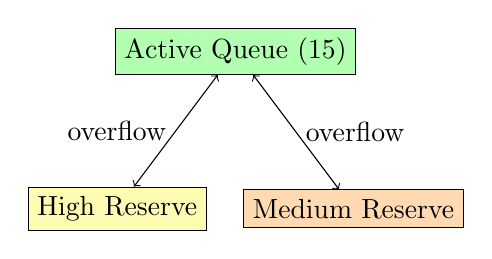
\begin{tikzpicture}[scale=1]
                \node[draw, rectangle, fill=green!30] (active) at (0,2) {Active Queue (15)};
                \node[draw, rectangle, fill=yellow!30] (high) at (-1.5,0) {High Reserve};
                \node[draw, rectangle, fill=orange!30] (med) at (1.5,0) {Medium Reserve};
                
                \draw[<->] (active) -- node[left] {overflow} (high);
                \draw[<->] (active) -- node[right] {overflow} (med);
            \end{tikzpicture}
        \end{column}
    \end{columns}
    
    \vspace{1em}
    \begin{evaluation}{Advantage}
        \begin{itemize}
            \item Prevents path explosion while maintaining security focus
        \end{itemize}
    \end{evaluation}
\end{frame}

\section{The Results}

\begin{frame}
    \frametitle{Evaluation Methodology}
    \begin{implementation}{Test Suite Design}
        \begin{itemize}
            \item \textbf{7 synthetic programs} targeting different challenges
            \item \textbf{Known vulnerabilities} with clear taint flow patterns
            \item \textbf{Controlled comparison:} TraceGuard vs. Classical Angr strategy
        \end{itemize}
    \end{implementation}
    
    \textbf{Programs Test:}
    \begin{itemize}
        \item Simple baselines, conditional explosions, deep exploration
        \item Multi-function analysis, perfect scenarios, recursive calls
        \item State explosion stress test
    \end{itemize}
\end{frame}

\begin{frame}
    \frametitle{Key Results - Execution Time Performance}
    \centering
    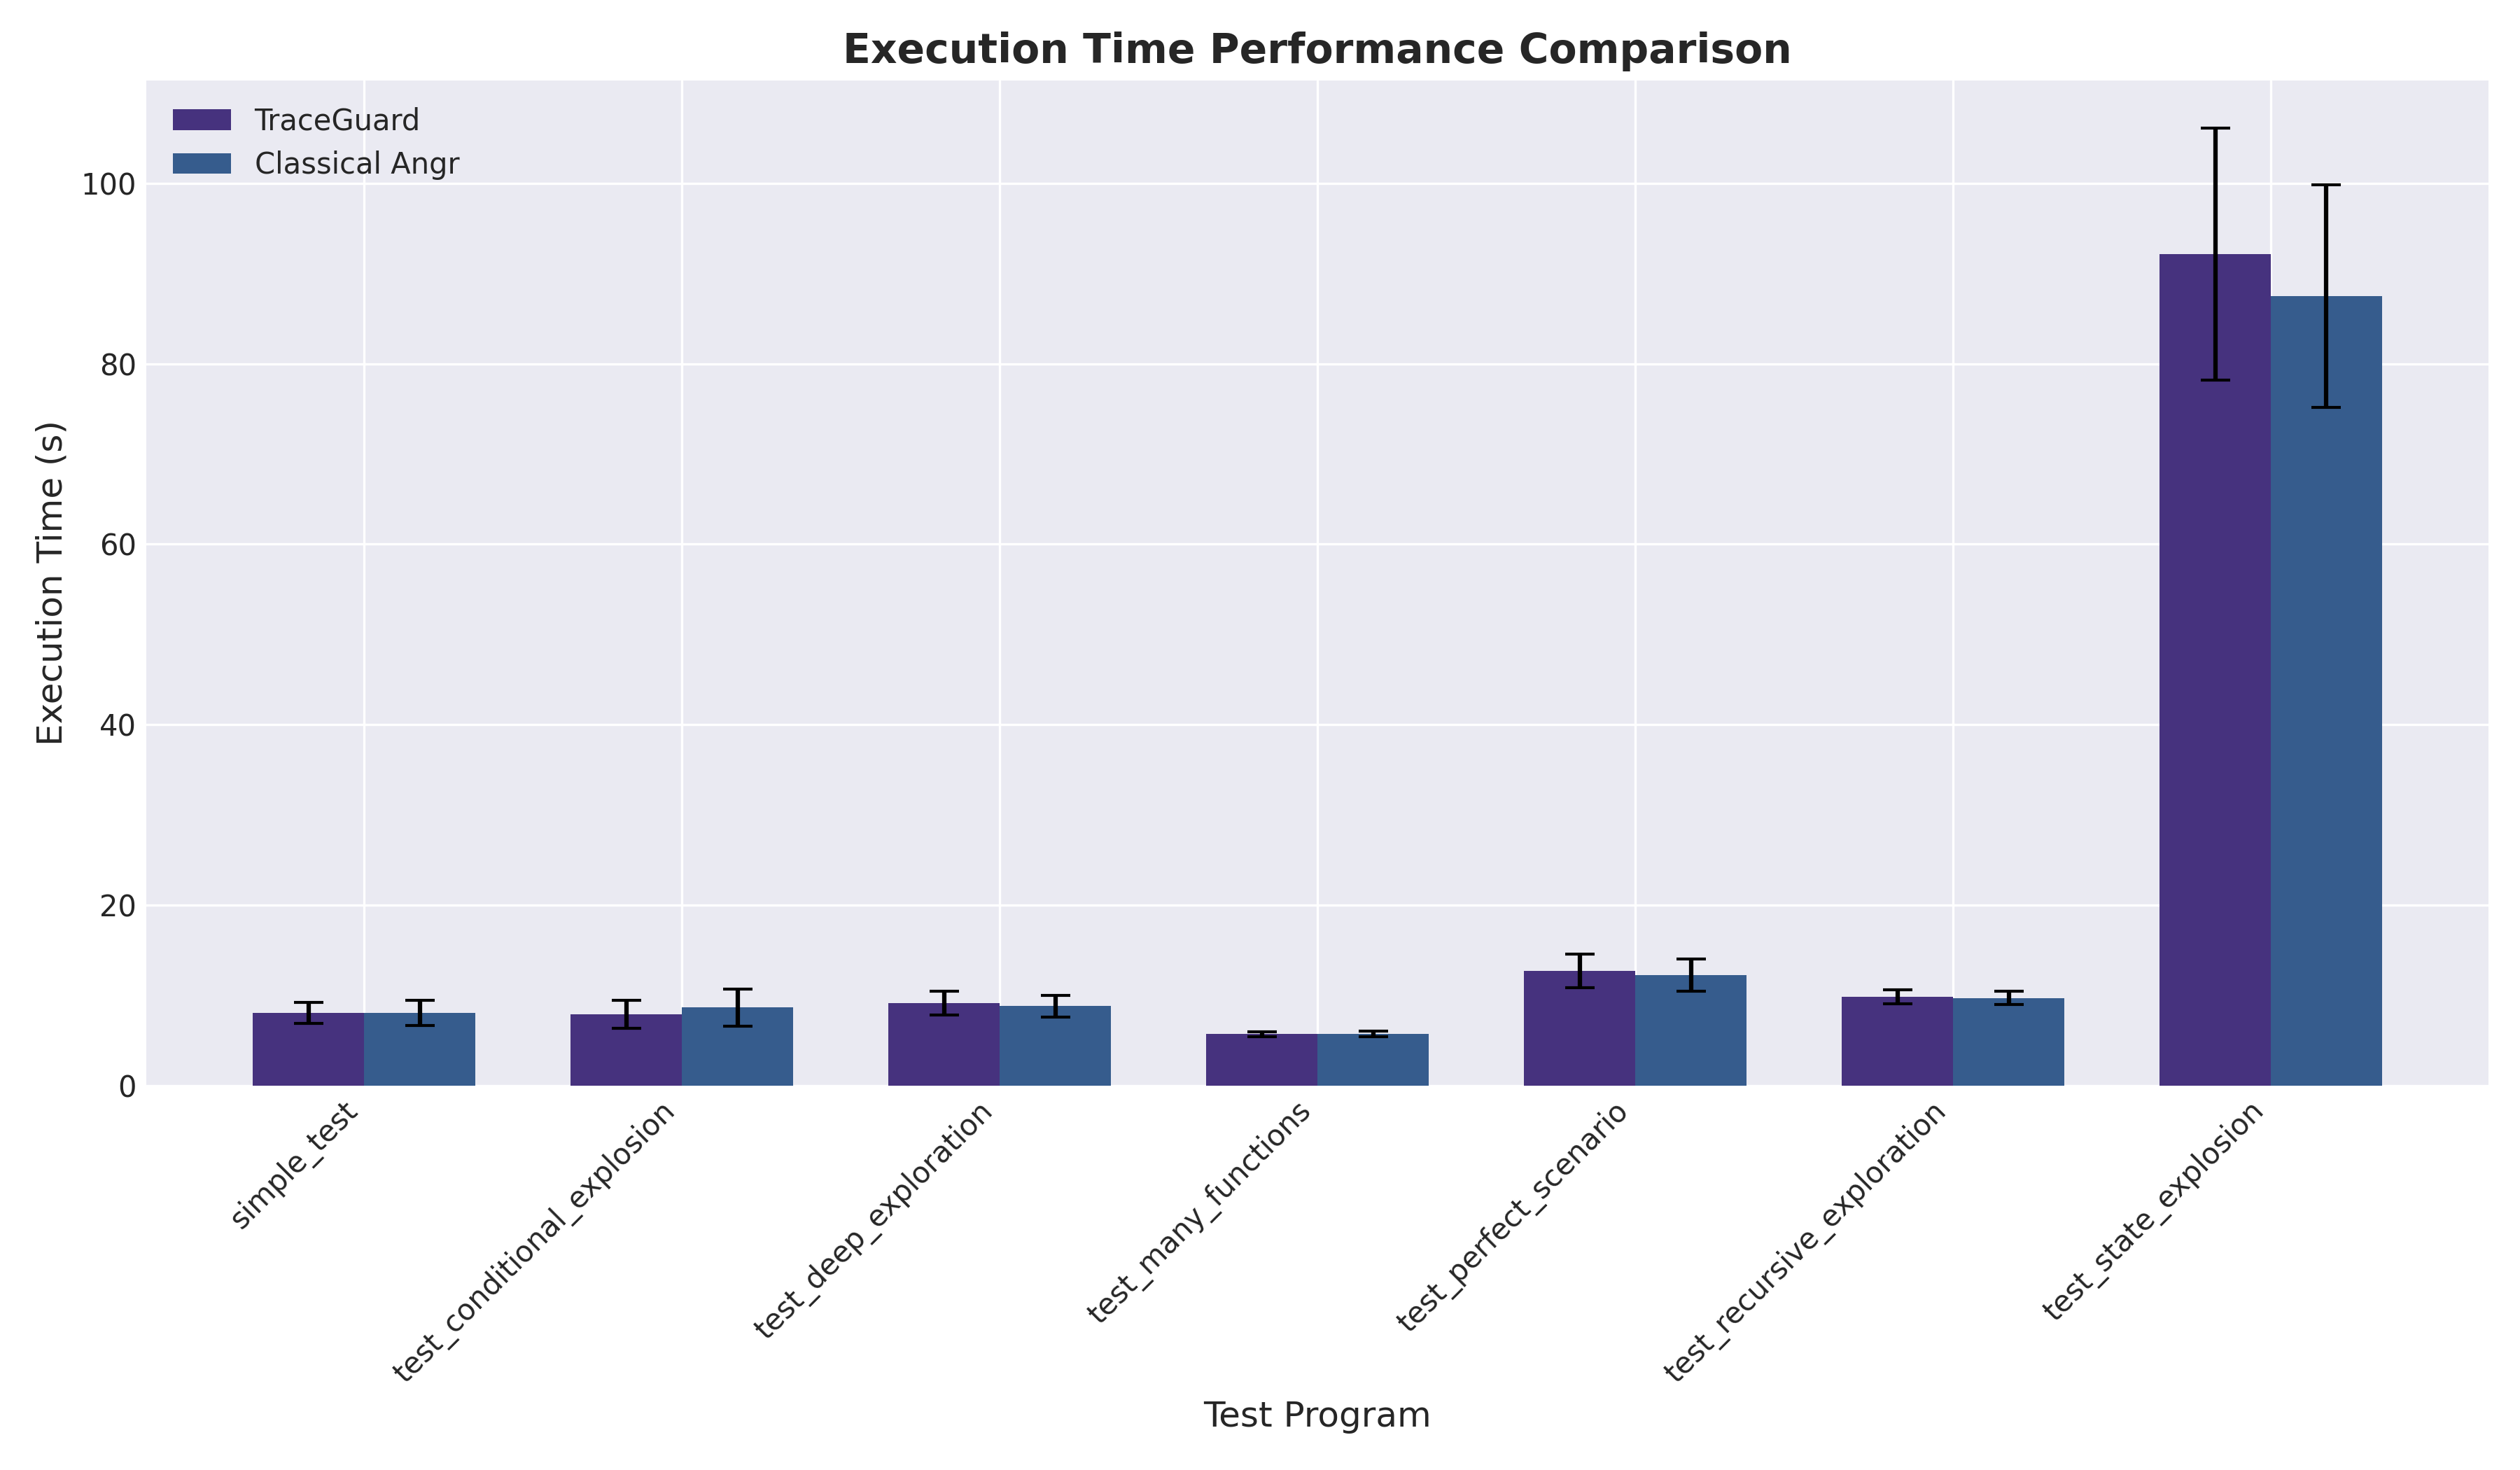
\includegraphics[width=0.95\textwidth]{./pic/execution_time_performance.png}
\end{frame}

\begin{frame}
    \frametitle{Key Results - Execution Time Performance}
    \begin{evaluation}{Key Insights}
        \begin{itemize}
            \item \textbf{Competitive Performance:} TraceGuard shows -5.3\% to +8.5\% time variation compared to Classical Angr. 
            \item \textbf{Complex Branching Improvement:} Achieved an 8.5\% time improvement in the \texttt{test\_conditional\_explosion} scenario. 
            \item \textbf{Scalability in Stress Test:} Maintained comparable execution time in the \texttt{test\_state\_explosion} scenario, despite its complexity. 
        \end{itemize}
    \end{evaluation}
\end{frame}

\begin{frame}
    \frametitle{Vulnerability Detection Effectiveness}
    \centering
    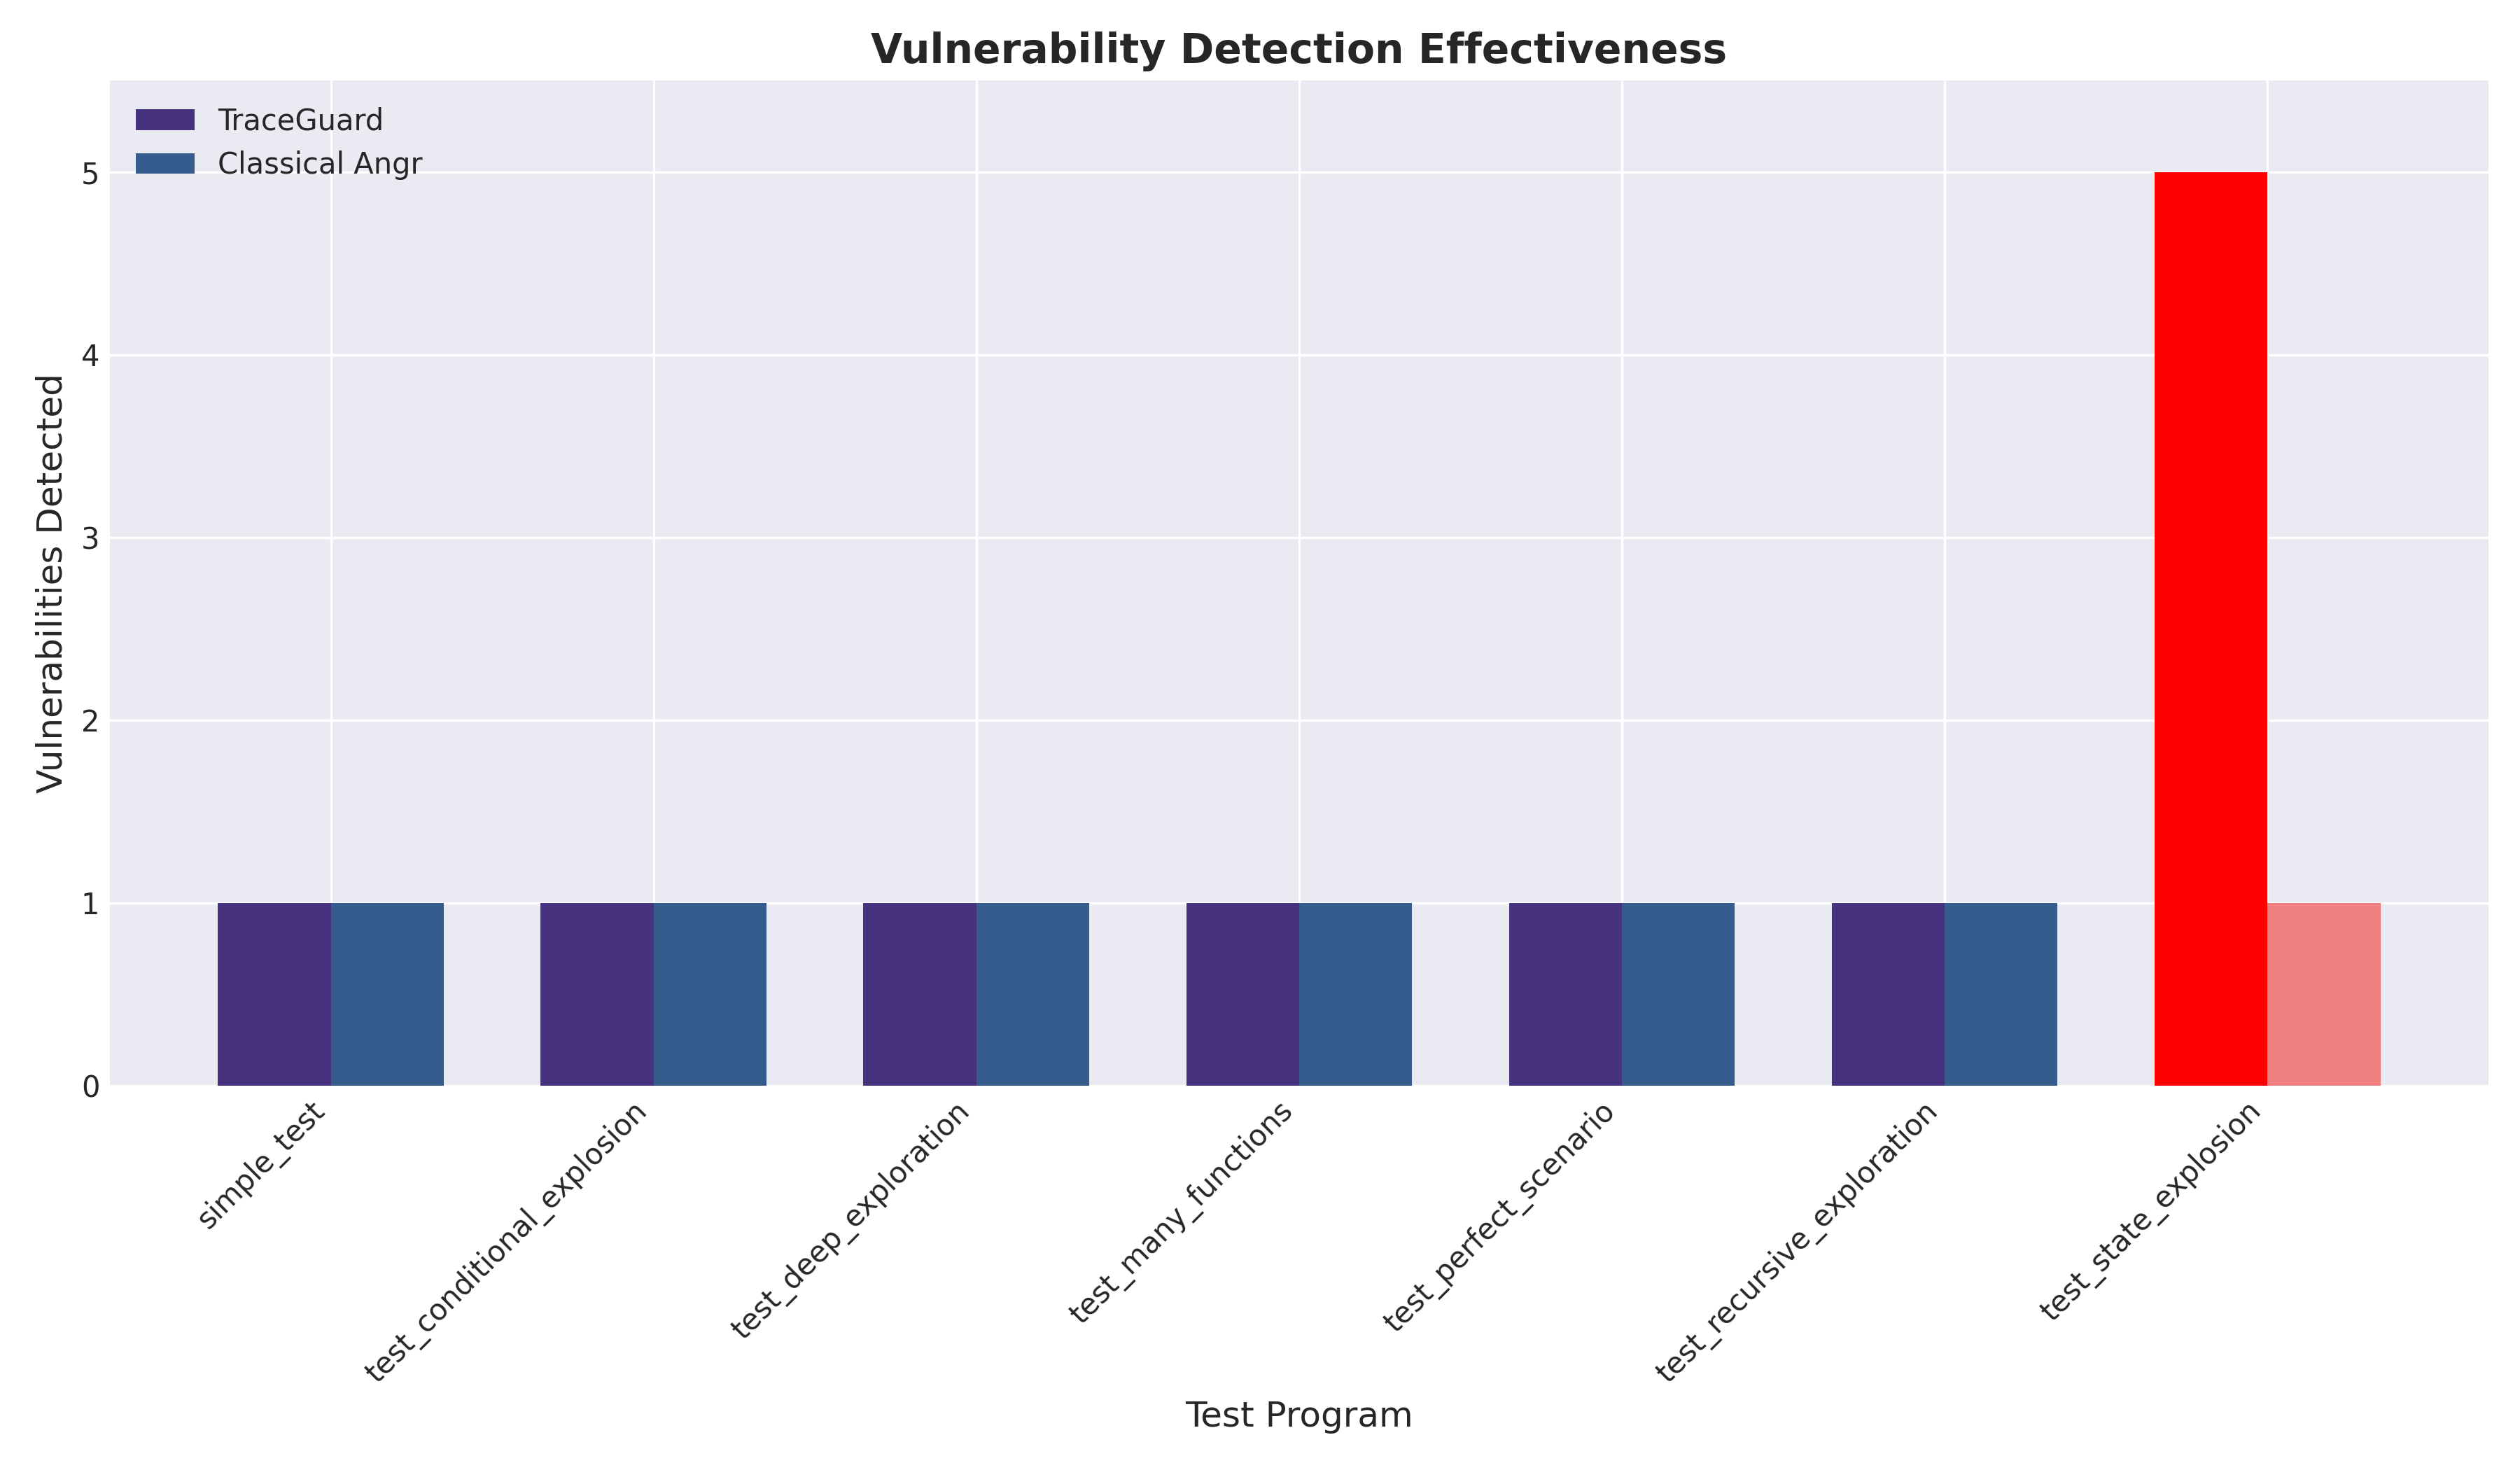
\includegraphics[width=0.95\textwidth]{./pic/vulnerability_detection_effectiveness.png}
\end{frame}

\begin{frame}
    \frametitle{Vulnerability Detection Effectiveness}
    \begin{evaluation}{Perfect Detection with Superior Performance}
        \begin{itemize}
            \item \textbf{100\% Vulnerability Coverage}
            \item \textbf{Strategic Advantage in Complexity:} TraceGuard found \textbf{$5 \times$ more vulnerabilities} in the challenging \texttt{test\_state\_explosion} scenario.
            \item \textbf{Consistent and Enhanced Reliability:} TraceGuard maintains consistent detection for all test types while providing a significant leap in highly complex environments.
        \end{itemize}
    \end{evaluation}
\end{frame}

\begin{frame}
    \frametitle{Coverage vs. Effectiveness}
    \centering
    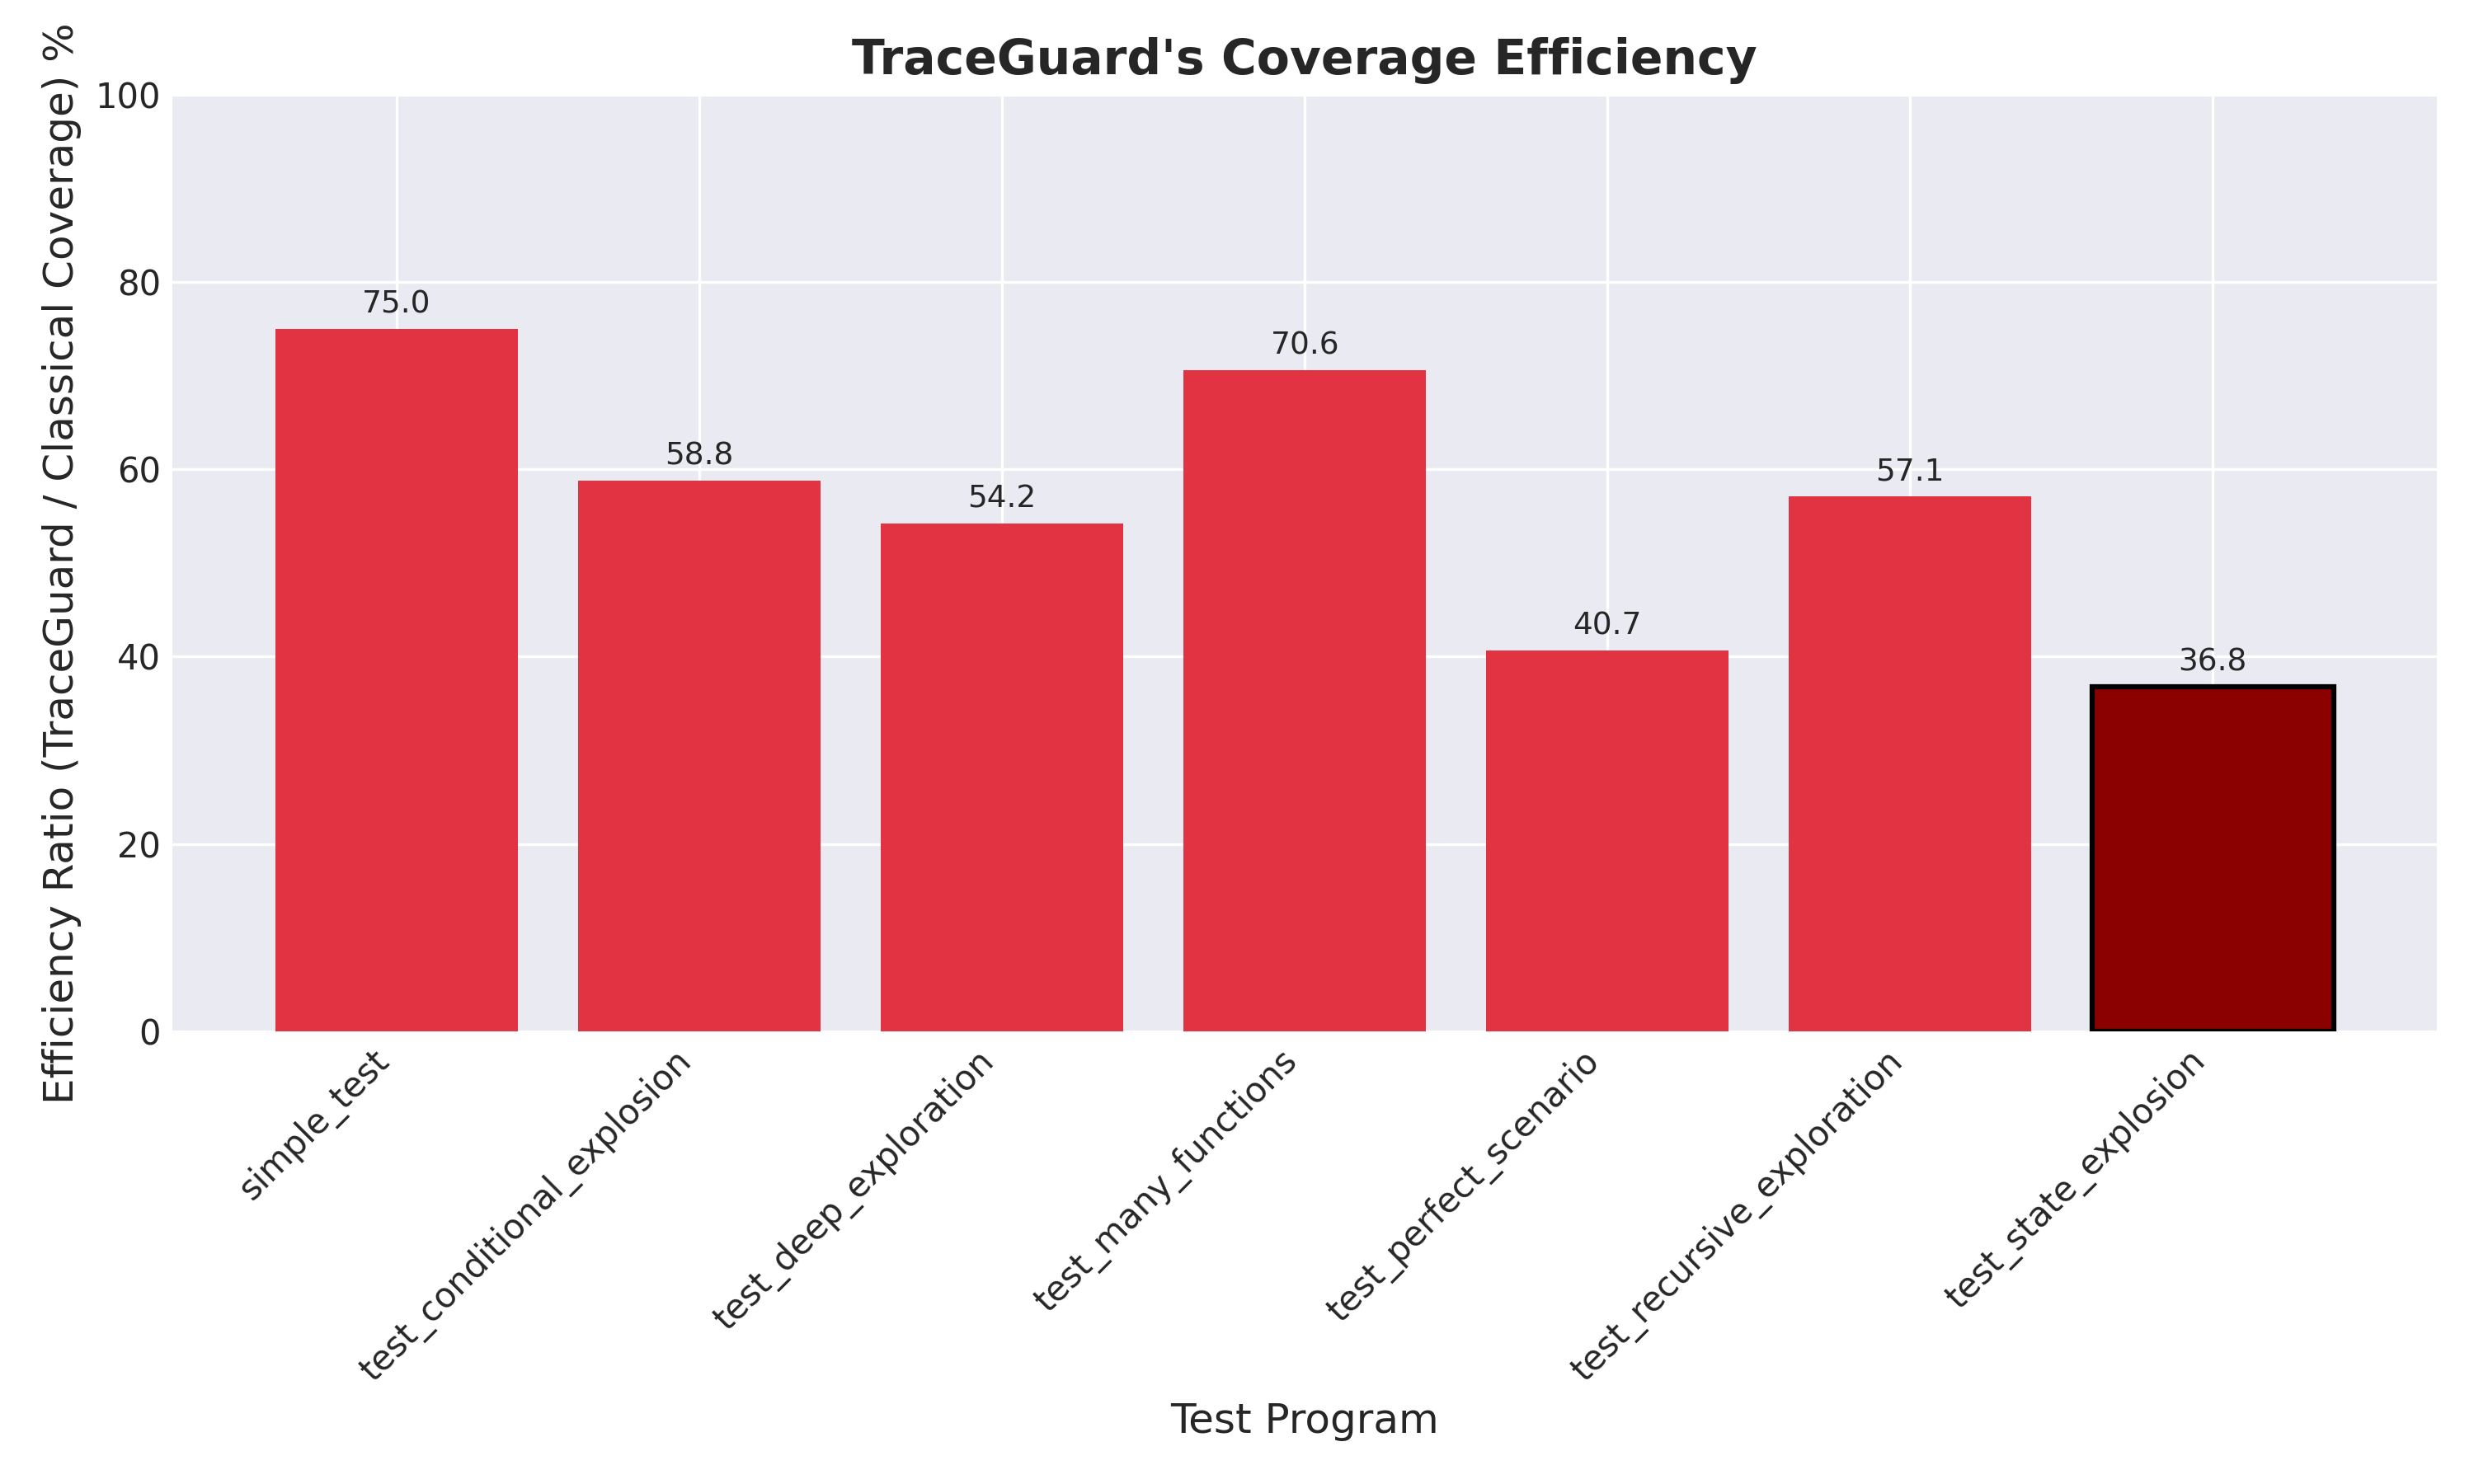
\includegraphics[width=0.95\textwidth]{./pic/coverage_efficiency.png}
\end{frame}

\begin{frame}
    \frametitle{Efficiency: Quality Over Quantity}
    \begin{evaluation}{Paradigm Shift}
        \begin{itemize}
            \item \textbf{Traditional Metric:} More coverage $\implies$ better analysis
            \item \textbf{Our Finding:} \alert{Focused exploration $\implies$ more critical vulnerabilities}
            \item \textbf{The Proof (Example: \texttt{test\_state\_explosion}):}
                  \begin{itemize}
                        \item TraceGuard found \textbf{$5 \times$ more vulnerabilities} with only \textbf{36.8\% of Classical's coverage}.
                  \end{itemize}
        \end{itemize}
    \end{evaluation}

    \vspace{0.5em}
    \begin{center}
        \large\textbf{\alert{Quality of exploration matters more than quantity}}
    \end{center}
\end{frame}

\section{Live Demo}

\begin{frame}
    \frametitle{Live Demo - TraceGuard in Action}
    \begin{implementation}{Demo Setup}
        \vspace{0.2em}
        \textbf{Target:} \texttt{examples/program6}
        
        \textbf{What we'll see:}
        \begin{enumerate}
            \item Taint source detection (fgets)
            \item Real-time taint propagation tracking
            \item Guided exploration prioritization
            \item Vulnerability discovery and reporting
            \item Interactive visualization
        \end{enumerate}
    \end{implementation}
    
    \begin{center}
        \Large\textbf{[LIVE DEMO]}
    \end{center}
\end{frame}

\section{Future Directions}

\begin{frame}
    \frametitle{Future Research Directions}
    \begin{columns}
        \begin{column}{0.5\textwidth}
            \textbf{Immediate Extensions:}
            \begin{itemize}
                \item \textbf{Real-world validation:} Large-scale commercial software
                \item \textbf{Enhanced taint sources:} Network protocols, file formats
                \item \textbf{Multi-architecture:} ARM, RISC-V support
                \item \textbf{Integration:} Fuzzing tools, static analysis
            \end{itemize}
        \end{column}
        \begin{column}{0.5\textwidth}
            \textbf{Advanced Research:}
            \begin{itemize}
                \item \textbf{Machine learning guidance:} AI-driven exploration
                \item \textbf{Distributed analysis:} Cloud-scale symbolic execution
                \item \textbf{Formal verification:} Soundness guarantees
                \item \textbf{Byte-level tracking:} Enhanced taint granularity
            \end{itemize}
        \end{column}
    \end{columns}
\end{frame}

\begin{frame}
    \frametitle{Broader Impact \& Applications}
    \begin{research}{Academic Impact}
        \begin{itemize}
            \item \textbf{Methodology:} Security-aware program analysis paradigm
            \item \textbf{Tool:} Open source platform for continued research
            \item \textbf{Validation:} Empirical evidence for taint-guided approaches
        \end{itemize}
    \end{research}
    
    \vspace{1em}
    \begin{implementation}{Industry Applications}
        \begin{itemize}
            \item \textbf{Security auditing:} Automated vulnerability discovery
            \item \textbf{DevSecOps:} Pre-deployment security testing
            \item \textbf{Penetration testing:} Target identification for manual analysis
            \item \textbf{Critical Infrastructure:} Security validation for high-stakes systems
        \end{itemize}
    \end{implementation}
\end{frame}

\section{Conclusion}

\begin{frame}
    \frametitle{Summary and Conclusion}
    \begin{evaluation}{What We Achieved}
        \begin{itemize}
            \item \textbf{Solved fundamental problem:} Path explosion in security analysis
            \item \textbf{Demonstrated effectiveness:} 100\% vulnerability detection, $5 \times$ improvement
            \item \textbf{Practical implementation:} Ready for real-world deployment
            \item \textbf{Research foundation:} Platform for future security-aware analysis
        \end{itemize}
    \end{evaluation}
    
    \begin{implementation}{Deployment Context}
        \begin{itemize}
            \item \textbf{Continuous Integration:} Automated security testing in CI/CD pipelines
            \item \textbf{Red Team Operations:} Efficient vulnerability discovery
            \item \textbf{Research Platform:} Foundation for advanced program analysis
        \end{itemize}
    \end{implementation}
\end{frame}

\begin{frame}
    \frametitle{Research Contributions}
    \begin{research}{Novel Integration}
        \begin{itemize}
            \item First comprehensive framework for real-time taint-guided symbolic execution
            \item Dynamic state prioritization based on security relevance
            \item Practical implementation demonstrating feasibility
        \end{itemize}
    \end{research}
    
    \vspace{1em}
    \begin{implementation}{Technical Achievements}
        \begin{itemize}
            \item Custom Angr exploration technique
            \item Function-level taint tracking system
            \item Adaptive scoring algorithm with configurable thresholds
            \item Comprehensive benchmarking infrastructure
        \end{itemize}
    \end{implementation}
\end{frame}

\section{Questions?}

\begin{frame}
    \frametitle{Thank You}
    \begin{center}
        \Large Questions and Discussion
        
        \vspace{2em}
        \normalsize
        \textbf{TraceGuard: Taint-Guided Symbolic Execution} \\
        for Enhanced Binary Analysis
        
        \vspace{1em}
        Ruben Hutter \\
        University of Basel \\
        Supervisor: Prof. Dr. Christopher Scherb
        
        \vspace{2em}
        \textbf{Available Resources:}
        \begin{itemize}
            \item \textbf{Live Tool:} github.com/ruben-hutter/TraceGuard
            \item \textbf{Thesis:} Full technical details and evaluation
            \item \textbf{Demo:} Additional scenarios and visualizations
        \end{itemize}
    \end{center}
\end{frame}

\end{document}
